% Adjust these for the path of the theme and its graphics, relative to this file
%\usepackage{beamerthemeFalmouthGamesAcademy}
\usepackage{../../beamerthemeFalmouthGamesAcademy}
\usepackage{multimedia}
\graphicspath{ {../../} }

\usepackage{textcomp}

% Default language for code listings
\lstset{language=Python, upquote=true,
        morekeywords={each,in,nullptr}
}

% For strikethrough effect
\usepackage[normalem]{ulem}
\usepackage{wasysym}

\usepackage{pdfpages}

% http://www.texample.net/tikz/examples/state-machine/
\usetikzlibrary{positioning, calc, shapes.geometric, shapes.multipart, 
	shapes, arrows.meta, arrows, 
	decorations.markings, external, trees, automata}

\setbeamertemplate{navigation symbols}{}

\newcommand{\fullbleed}[1]{
\begin{frame}[plain]
	\begin{tikzpicture}[remember picture, overlay]
		\node[at=(current page.center)] {
			\includegraphics[width=\paperwidth]{#1}
		};
	\end{tikzpicture}
\end{frame}
}

\newcommand{\picturepage}[2]{
\begin{frame}[plain]
	\begin{tikzpicture}[remember picture, overlay]
		\node[at=(current page.center)] {
			\includegraphics[width=\paperwidth]{#1}
		};
		\draw<1>[draw=none, fill=black, opacity=0.9] (-1,-5.2) rectangle (current page.south east);
		\node[draw=none,text width=0.96\paperwidth, align=right] at (5.5,-5.5) {\tiny{#2}};
	\end{tikzpicture}
\end{frame}
}

\newcommand{\notepicx}[5]{
\begin{frame}[plain]
	\begin{tikzpicture}[remember picture, overlay]
		\node[at=(current page.center)] {
			\includegraphics[width=\paperwidth]{#1}
		};
		\node[draw=none, fill=black, text width=#5\paperwidth] at ([xshift=#3, yshift=#4] current page.center) {\small{#2}};
	\end{tikzpicture}
\end{frame}
}

\newcommand{\notepic}[4]{
	\notepicx{#1}{#2}{#3}{#4}{0.4}
}

\begin{document}
\title{\sessionnumber: Tinkering Graphics II}
\subtitle{\modulecode: \moduletitle}

\frame{\titlepage} 

\begin{frame}
	\frametitle{Learning Outcomes}
	\begin{itemize}
		%\item \textbf{Analyse} the role of computing professionals in the games industry
		%Comp110 - 02 Material and Tinkering Text
%		\item \textbf{Apply} pair programming practices to solve a simple problem
		\item\textbf{Explain and translate} technical notation for algorithms
		\item\textbf{Trace} some code using debugging tools
	\end{itemize}
\end{frame}

\part{Code Tracing}
\frame{\partpage}

\begin{frame}
\frametitle{Demo}
\noindent We will begin this class with a quiz.  
We wish to develop a program that takes a sequence of ASCII characters 
	and outputs a frequency-sorted concordance of all words in the input.\\
We define a word with the following regular expression: [A-Za-z]+ \\
Words must be bounded by white space.
\end{frame}

\begin{frame}
\frametitle{Demo}
An example usage of our program is:
\begin{center}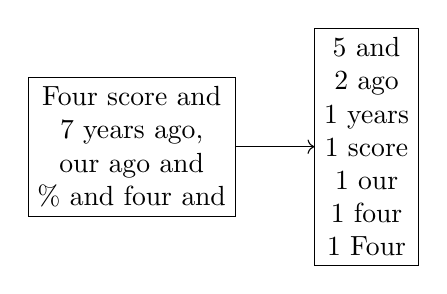
\begin{tikzpicture}
	% input
		\node[rectangle, draw, align=center] (input) 
			{Four score and \\ 7 years ago, \\ our ago and \\ \% and four and};
	% output
		\node[rectangle, draw, right =of input, align=center] (output) 
			{5 and \\ 2 ago \\ 1 years \\ 1 score \\ 1 our \\ 1 four \\ 1 Four};
	% arrow
		\draw [->] (input.east) -- (output.west);
\end{tikzpicture}\end{center}
\end{frame}

\begin{frame}
\frametitle{Demo}
\noindent This was used by Turing Award winner DE Knuth as press for his book, 
	\underline{The Art of Computer Programming} \\
The motivation came from difficulties in creating the initial press for his book;\\
	\indent The lead type press could not handle code or equations, which were fundamental! \\
So Knuth invented a language to produce correct images, called Tex. \\
He developed a textbook to bring attention to his language, which explained the framework.
\end{frame}

\begin{frame}
\frametitle{Demo}
The framework took the form:
\begin{center}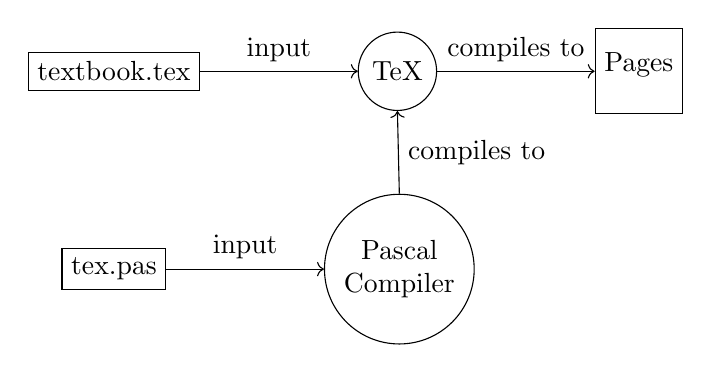
\begin{tikzpicture}
	\node[rectangle, draw] (book) {textbook.tex};
	\node[rectangle, draw, below =2cm of book] (pas) {tex.pas};
	\node[circle, draw, right =2cm of book] (TeX) {TeX};
	\node[circle, draw, right =2cm of pas, align=center] (P) {Pascal\\Compiler};	
	\node[rectangle, draw, right =2cm of TeX, align=center] (Pages) {\\Pages\\};		
	\draw [->] (book.east) -- node [align=center, above] {input} (TeX.west);
	\draw [->] (pas.east) -- node [align=center, above] {input} (P.west);
	\draw [->] (P.north) -- node [align=center, right] {compiles to} (TeX.south);		
	\draw [->] (TeX.east) -- node [align=center, above] {compiles to} (Pages.west);	
\end{tikzpicture}\end{center}
\noindent This presents a large (and common) issue --  code and documentation must be kept in agreement.\\
Knuth developed the idea of a unified, interleaved file to combat this.
\end{frame}

\begin{frame}
\frametitle{Demo}
Thus his program took the following final form:\\
\resizebox{\textwidth}{!}{%
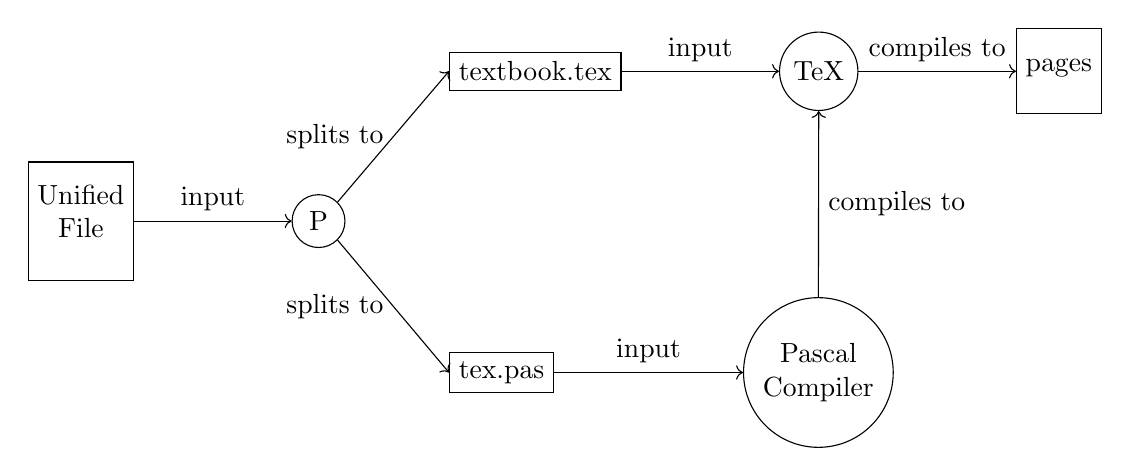
\begin{tikzpicture}
	% nodes
		\node[rectangle, draw, align=center] (unified) {\\Unified\\File\\};
		\node[circle, draw, right =2cm of unified, align=center] (splitter) {P};	
		\node[rectangle, draw, above right =2cm of splitter] (book) {textbook.tex};
		\node[rectangle, draw, below right =2cm of splitter] (pas) {tex.pas};
		\node[circle, draw, right =2cm of book] (TeX) {TeX};
		\node[circle, draw, right =2.4cm of pas, align=center] (P) {Pascal\\Compiler};	
		\node[rectangle, draw, right =2cm of TeX, align=center] (pages) {\\pages\\};
	%edges 
		\draw [->] (unified.east) -- node [align=center, above] {input} (splitter.west);
		\draw [->] (splitter.north east) -- node [align=center, left] {splits to} (book.west);
		\draw [->] (splitter.south east) -- node [align=center, left] {splits to} (pas.west);
		\draw [->] (book.east) -- node [align=center, above] {input} (TeX.west);
		\draw [->] (pas.east) -- node [align=center, above] {input} (P.west);
		\draw [->] (P.north) -- node [align=center, right] {compiles to} (TeX.south);		
		\draw [->] (TeX.east) -- node [align=center, above] {compiles to} (pages.west);	
\end{tikzpicture}
}%
\end{frame}

\begin{frame}
\frametitle{Demo}
\noindent This left him with a nearly 500 page textbook; how would he drum up interest?\\
Like a good computer scientist, he chose to write a paper.\\
He coined his approach \textbf{\underline{literate programming}}.\\
This has become standard practice in many disciplines; we can see JavaLibrary for proof.\\ 
Knuth approached Doug McIlroy, the manager for the development of UNIX, for help.\\
McIlroy suggested our problem as an example\\
Knuth wrote a solution using Hash Tries via literate programming!\\
Running it through TeX gives pages and through pascal gives the paper!
\end{frame}

\begin{frame}
\frametitle{Demo}
\noindent As impressive as this was, the afterword was what stuck.\\
McIlroy proposed the following trivial BASH solution (he was the brain behind UNIX pipes after all)
%	\begin{lstlisting}
%	tr -c 'A-Za-z' '\n' | sort | uniq -c | sort -rn
%	\end{lstlisting}
The pascal solution was, say, 1000 lines.\\
\indent It was faster\\
\indent It was more "checked" by compilers\\
BUT the bash solution is exceedingly simple and documents itself as follows:
\begin{center}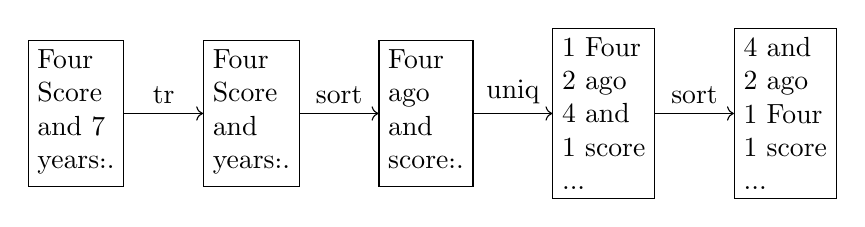
\begin{tikzpicture}
	\node[rectangle, draw, align=left] (1) {Four\\Score\\and 7\\years\...};
	\node[rectangle, draw, align=left, right =of 1] (2) {Four\\Score\\and\\years\...};
	\node[rectangle, draw, align=left, right =of 2] (3) {Four\\ago\\and\\score\...};
	\node[rectangle, draw, align=left, right =of 3] (4) {1 Four\\2 ago\\4 and\\1 score\\...};
	\node[rectangle, draw, align=left, right =of 4] (5) {4 and\\2 ago\\1 Four\\1 score\\...};
	\draw [->] (1.east) -- node [align=center, above] {tr} (2.west);
	\draw [->] (2.east) -- node [align=center, above] {sort} (3.west);
	\draw [->] (3.east) -- node [align=center, above] {uniq} (4.west);
	\draw [->] (4.east) -- node [align=center, above] {sort} (5.west);
\end{tikzpicture}\end{center}
\end{frame}

\begin{frame}
\frametitle{Demo}
\noindent This demonstrates an issue fundamental to computer science called \textbf{\underline{choice of notation}}.\\
There are pros and cons to any choice of notation, and it is up to the engineer to weigh them!\\
As this is a discussion of languages, consider the following fundamental linguistic hypothesis:\\
\textbf{\underline{Sapir-Whorf Hypothesis}}. \begin{itemize}
\item There is no limit on the structural diversity of language.
\item The structure of a language determines a native speaker's perception of experience.
\end{itemize}
This was proposed by linguists for natural languages, but (b) was softened. Even though it is false, it stuck: see “Eskimos have 19 words for snow”. Even if false for natural languages,  it is true for programming languages!
\end{frame}


\part{Code Tracing}
\frame{\partpage}

\begin{frame}
\frametitle{Demo}

\begin{itemize}		
	\item Start using debug tools when you run into problems:
	\item \url{https://www.youtube.com/watch?v=QJtWxm12Eo0}
\end{itemize}

\end{frame}

\begin{frame}[fragile]
	\frametitle{Source Code: Less Red}
	
\begin{lstlisting}
def decreaseRed(picture, amount):
  pixelMatrix = getPixels(picture)
  for pixel in pixelMatrix:
    value = getRed(pixel)
    setRedPixel(pixel, value * amount)
\end{lstlisting}

Note: This source code excerpt will not work in PyGame.

\end{frame}

\fullbleed{big_ben}

\begin{frame}{Activity: Less Red}
	\vspace{2em}
	
	If `bb' is the original picture of Big Ben, which of the below function calls created the change:
	
	\begin{itemize}
		\item changeRed(bb, 1.5)
		\item changeRed(bb, 2.0)
		\item changeRed(bb, 0)
	\end{itemize}
\end{frame}

\part{PASS Challenge}
\frame{\partpage}

\begin{frame}
	\frametitle{PASS Challenge}
	
	Review the WAVE and PyGame mixer modules at:
	
	\url{https://docs.python.org/3.6/library/wave.html}
	
	\vspace{1em}
	
	\url{https://www.pygame.org/docs/ref/mixer.html}
\end{frame}	
	
\begin{frame}	
	\frametitle{PASS Challenge}
	\begin{itemize}
		\item In pairs
		\item \textbf{Implement} audio i/o in Python
		\item \textbf{Read} a wave file as a wave\_read object
		\item \textbf{Play} audio in PyGame using the PyGame Mixer
		\item \textbf{Write} a new wave file as a wave\_write object
	\end{itemize}
	
	You can learn more about audio:
	
	\vspace{1em}
	
	 \url{https://inventwithpython.com/chapter19.html}
	
\end{frame}

\end{document}